\subsection{Eksempel}
Gennemgangen af metoden er beskrevet i detalje for hver del, men det kan være svært at få overblikket over metoden.
Af denne grund gives her et eksempel, der tager en fra de rå data og hele vejen til det aggregerede resultat.
Eksemplet, der følges kan ses i \cref{fig:totalbanjo}.
%intro godt at give et eksempel
%gennemgang af hvert led
%resultatet er at man har regnet ud der soves derfra og dertil
\begin{figure}
	\begin{minipage}{\linewidth}
		\begin{subfigure}{0.5\linewidth}
			\centering
			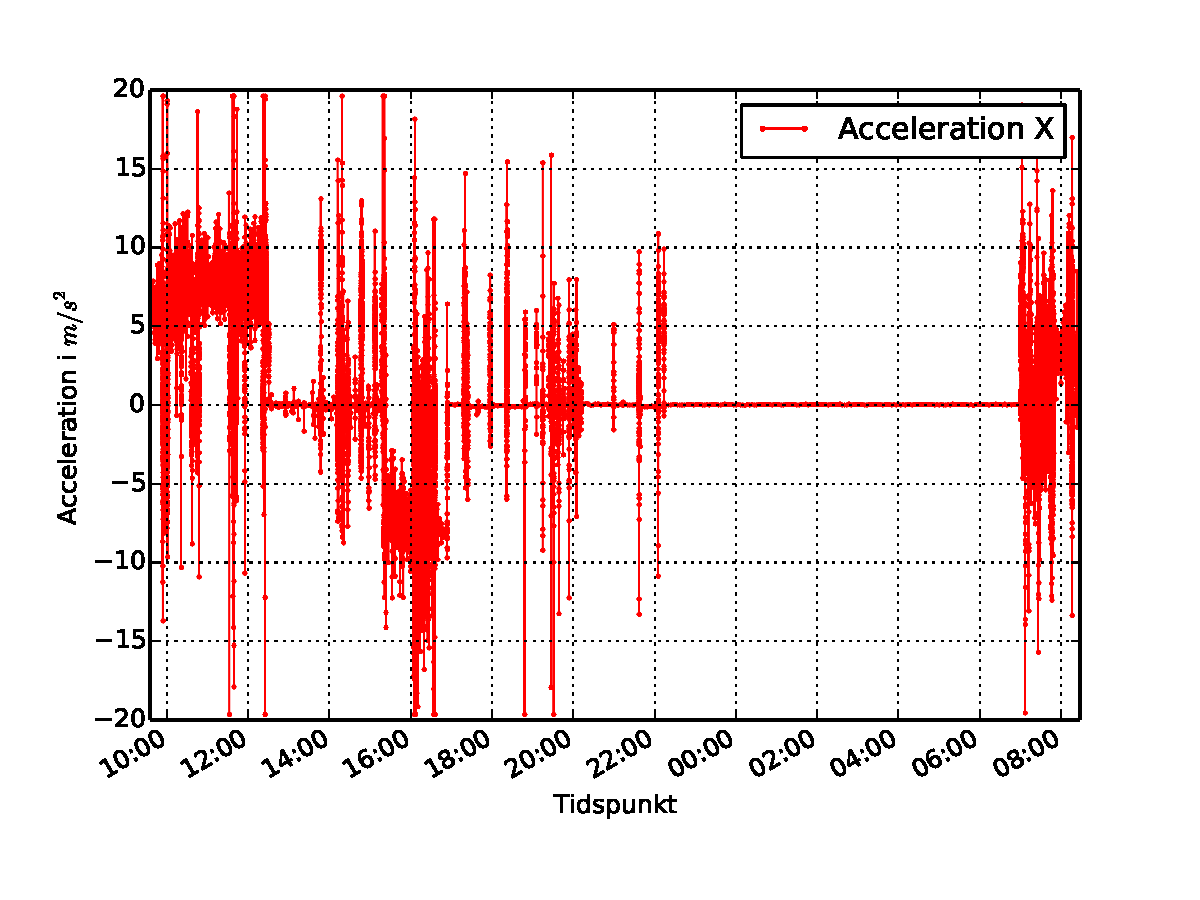
\includegraphics[scale=0.4, trim = 1cm 1cm 1cm 1cm, clip]{kombi_figur/acceleration-plot}
			\caption{Rå accelerations-data.}\label{fig:rawaccplot}
		\end{subfigure}
		\begin{subfigure}{0.5\linewidth}
			\centering
			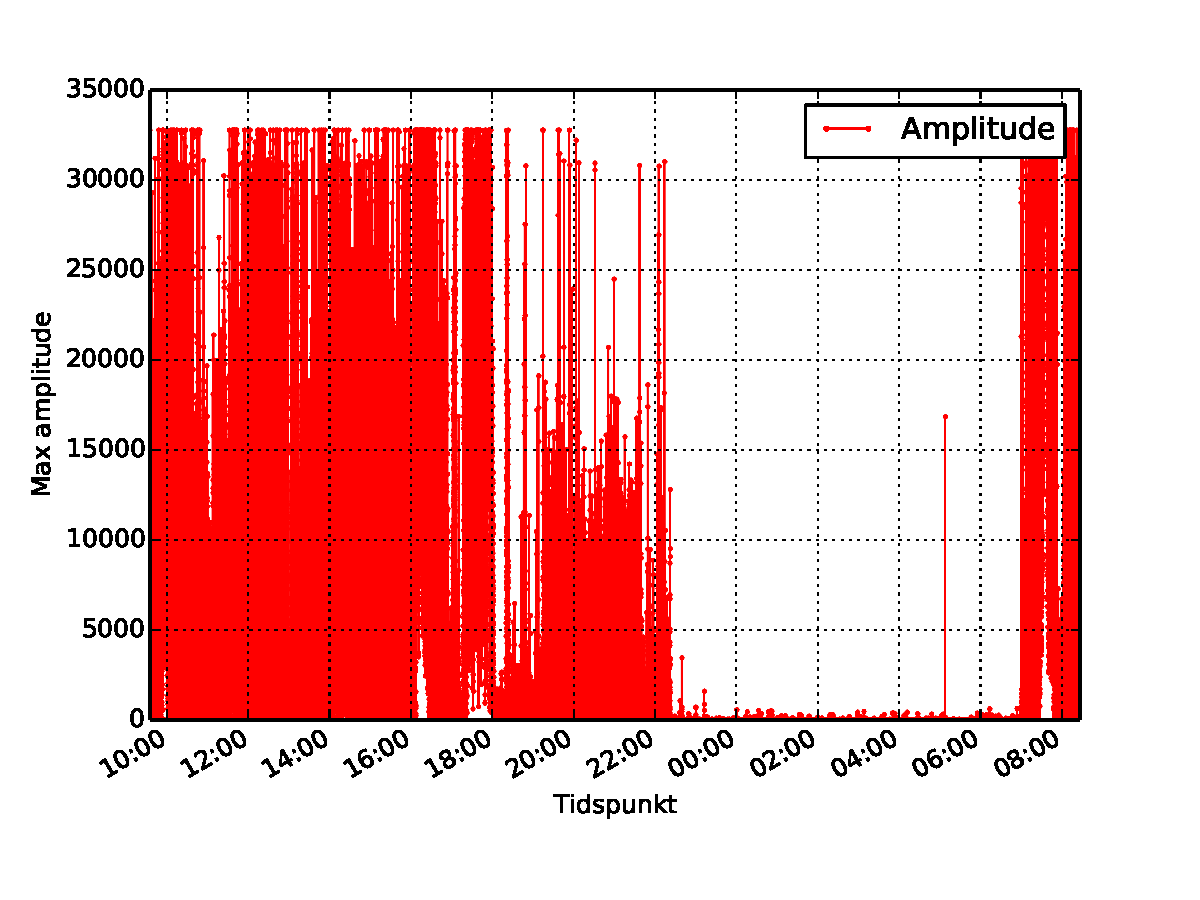
\includegraphics[scale=0.4, trim = 0cm 1cm 1cm 1cm, clip]{kombi_figur/amplitude-plot}
			\caption{Rå amplitude-data.}\label{fig:rawamplplot}
		\end{subfigure}
	\end{minipage}\\[1ex]%
	\begin{minipage}{\linewidth}
		\begin{subfigure}{0.5\linewidth}
			\centering
			
\includegraphics[scale=0.3, angle=270]{arrow}
		\end{subfigure}
		\begin{subfigure}{0.5\linewidth}
			\centering
			
\includegraphics[scale=0.3, angle=270]{arrow}
		\end{subfigure}
	\end{minipage}\\[1ex]%
	\begin{minipage}{\linewidth}
		\begin{subfigure}{0.5\linewidth}
			\centering
			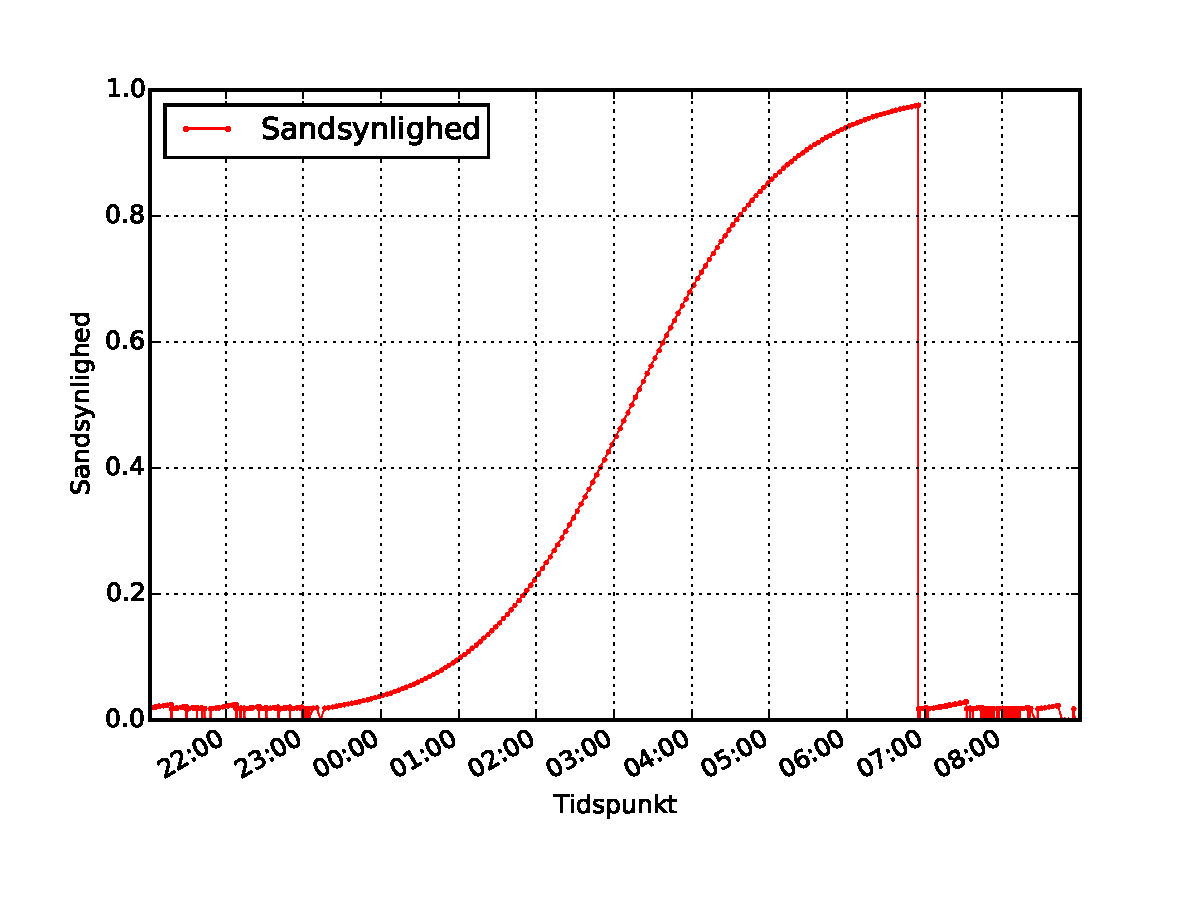
\includegraphics[scale=0.4, trim = 1cm 1cm 1cm 1cm, clip]{kombi_figur/acceleration-sleep-estimate-plot}
			\caption{Accelerations-søvnestimering.}\label{fig:sleepcalcaccplot}
		\end{subfigure}
		\begin{subfigure}{0.5\linewidth}
			\centering
			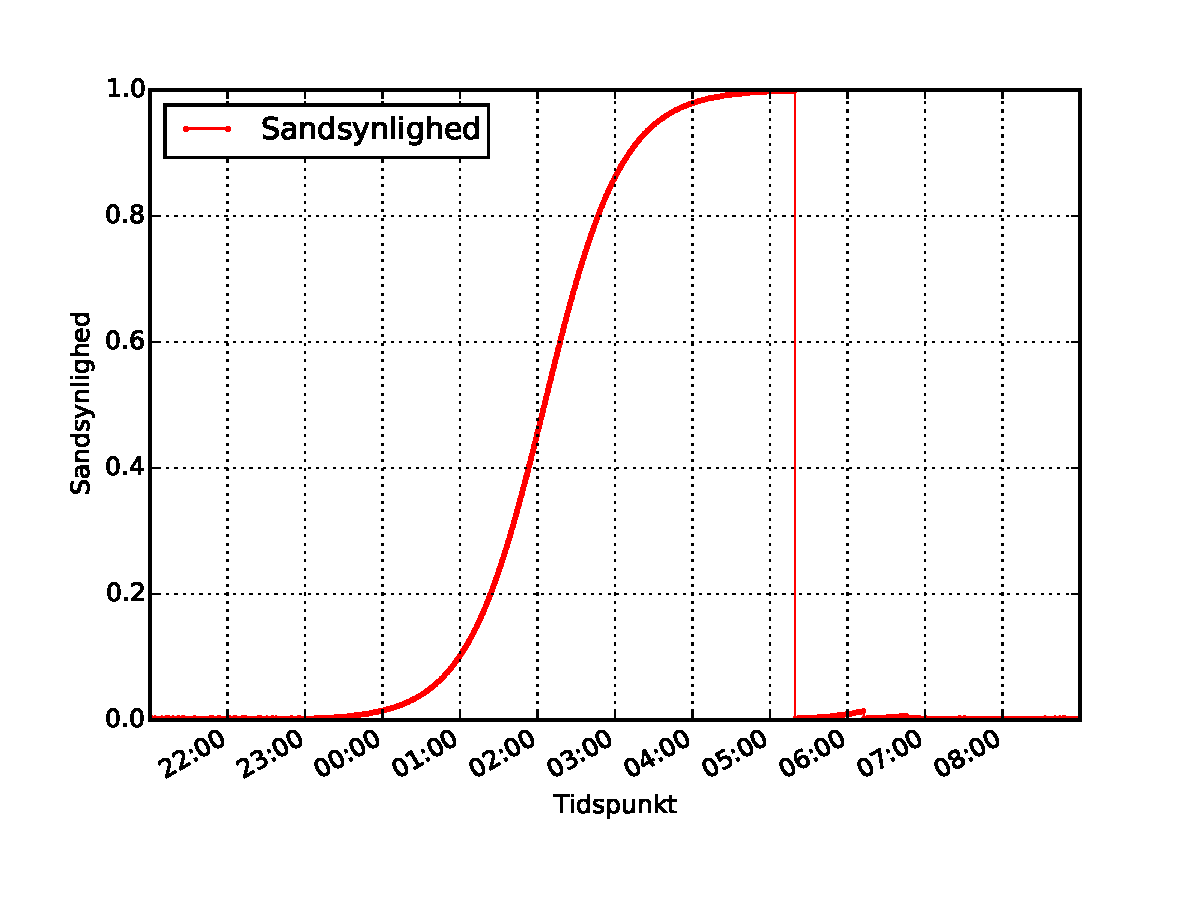
\includegraphics[scale=0.4, trim = 0cm 1cm 1cm 1cm, clip]{kombi_figur/amplitude-sleep-estimate-plot}
			\caption{Amplitude-søvnestimering}\label{fig:sleepcalcamplplot}
		\end{subfigure}
	\end{minipage}\\[1ex]%
	\begin{minipage}{\linewidth}
		\begin{subfigure}{0.5\linewidth}
			\centering
			
\includegraphics[scale=0.2]{downarrow}
		\end{subfigure}
		\begin{subfigure}{0.5\linewidth}
			\centering
			
\includegraphics[scale=0.2,angle=180]{uparrow}
		\end{subfigure}
	\end{minipage}\\[1ex]%
	\begin{minipage}{\linewidth}
		\begin{subfigure}{\linewidth}
			\centering
			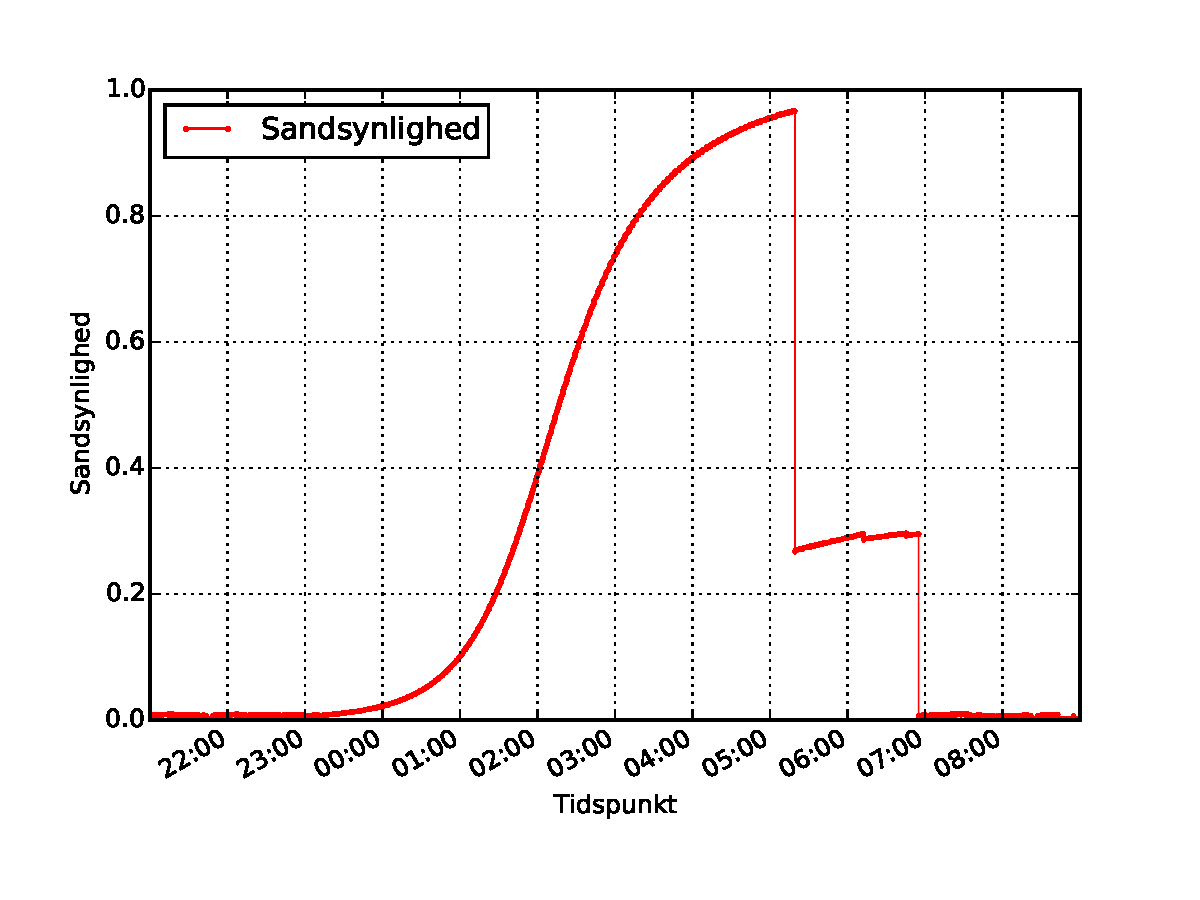
\includegraphics[scale=0.4, trim = 1cm 1cm 1cm 1cm, clip]{kombi_figur/combined-sleep-estimate-plot}
			\caption{Kombineret søvnestimering}\label{fig:sleepcalcombine}
		\end{subfigure}
	\end{minipage}\\[1ex]%
	\begin{minipage}{\linewidth}
		\begin{subfigure}{\linewidth}
			\centering
			
\includegraphics[scale=0.3, angle=270]{arrow}
		\end{subfigure}
	\end{minipage}\\[1ex]%
	\begin{minipage}{\linewidth}
		\begin{subfigure}{\linewidth}
			\centering
			\begin{tabular}{|c|c|c|}
			\hline starttid & sluttid & sandsynlighed \\ 
			\hline 2015-04-21 23:11 & 2015-04-22 05:19 & 0.97 \\ 
			\hline 2015-04-22 05:19 & 2015-04-22 06.45 & 0.29 \\ 
			\hline 
			\end{tabular}
			\caption{Samlet søvnaggregeringsresultat.}\label{fig:finalagg}
		\end{subfigure}
	\end{minipage}
	\caption{Illustration af søvnestimering fra rå data til aggregering.}\label{fig:totalbanjo}
\end{figure}

Der startes med de rå accelerations- og amplitude-data, der kan ses i \cref{fig:rawaccplot} og \cref{fig:rawamplplot}.
På dette datasæt foretages de beskrevne metoder, hvilket inkluderer et glidende gennemsnit, stilstandsbestemmelse og anvendelse af den logistiske funktion.
Hvis man ser på de rå accelerationsdata, \cref{fig:rawaccplot}, indikerer de at der er sovet omkring kl. 23 til lidt før kl. 7 næste dag.
Derimod hvis der ses på amplitudedata, \cref{fig:rawamplplot}, indikeres der samme periode, men hvor der har været larm kl. 05:19.
Dette skyldtes faktisk at en kat gik ind i soveværelset på pågældende tidspunkt.

Ved brug af de omtalte metoder på de rå datasæt, fås to separate søvnestimater, et fra accelerationsdata og et fra amplitudedata, der kan ses i \cref{fig:sleepcalcaccplot} og \cref{fig:sleepcalcamplplot}.
Vi observerer at acceleration-søvnestimeringen vokser helt frem til lidt før kl. 7.
Derimod ved amplitude-søvnestimeringen falder denne kl. 5:19 pga. larmen fra katten.
 
Herefter skal en kombinering laves af disse estimater, hvilket bliver udført ved hjælp af det vægtede gennemsnit.
Som resultat deraf fås et estimat, som kan ses i \cref{fig:sleepcalcombine}.
Da dette estimat er et vægtet gennemsnit af de enkelte søvnestimater, kan der ses hvordan sandsynligheden for at man sover falder efter kl. 05:19.
Dette behøver ikke være en ulempe for vores søvnestimat, da man godt kan forestille sig at søvnen er blevet forstyrret ved at katten gik ind i soveværelset.

Den kombinerede søvnestimering er basis for aggregeringen, som skal foretages til at registrere hvorfra og hvortil man har sovet, og er det endelige resultat, hvilket kan ses i \cref{fig:finalagg}.
Resultatet af aggregeringen afspejler fint de forudgående estimeringer, hvor man er væsentligt mere sikker på søvn inden katteforstyrrelsen kl. 05:19.